\chapter{Beta Function}
\minitoc
In this chapter, we discuss the Beta function related functions, namely, Beta Fucntion and incomplete Beta function.

\section{Beta Function}
The Beta function is definted in terms of the Gamma function:
\[ B(x, y) = \frac{\Gamma(x)\Gamma(y)}{\Gamma(x + y)} = \int_0^1 t^{x-1}(1-t)^{y-1}dt\]
for $x > 0$ and $y > 0$. Here are some basic facts about the beta function:
\begin{enumerate}
\item Beta function is symmetric, $B(x, y) = B(y, x)$.
\item For any real x in the domain, $\Gamma(x) = x\Gamma(x-1)$.
\item For any real x in the domain, 
\[\Gamma(1 - x)\Gamma(x) = \frac{\pi}{sin(\pi x)}\] 
This is called Euler's reflection and can be used to compute gamma function values for negative x if we know the values for positive x.
\end{enumerate} 
The graph for the beta function is below.
\begin{figure*}[htp]
\begin{center}
{
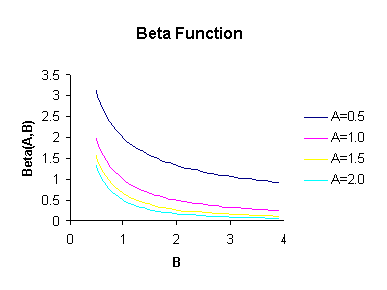
\includegraphics[bb=0 0 480 300,width=1\textwidth] {chap4/beta.png}
}
\end{center}
\caption{Incomplete Beta Function, from Boost}
\label{figure:betafunction}
\end{figure*}

\section{Incomplete Beta Function}
The incomplete Beta function is defined as
\[ B(x; a, b) = \int_0^x t^{a-1}(1-t)^{b-1}dt\]
for $a > 0$, $b > 0$, and $0 < x < 1$. The regularized incomplete Beta function is defined as
\[ I_x(a, b) = \frac{B(x; a, b)}{B(a, b)}\]
similar to the case of incomplete gamma function. Similarly, we could define the complementary regulaized incomplete beta function.
Here are some basica facts about the incomplete beta function:

The graph is below
\begin{figure*}[htp]
\begin{center}
{
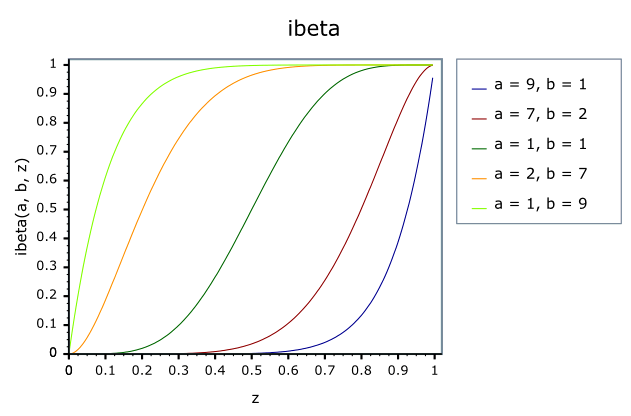
\includegraphics[bb=0 0 480 300,width=1\textwidth] {chap4/inbeta.png}
}
\end{center}
\caption{Incomplete Beta Function, from Boost}
\label{figure:incompletebetafunction}
\end{figure*}

\begin{thebibliography}{99}

% >>>>>>>>> Book examples <<<<<<<<<
\bibitem{Demmel@1997} Demmel, J.W., {\itshape Applied Numerical Linear Algebra},
 SIAM, 1997.
\bibitem{GolubLoan} Golub, G.H., Loan, C.F., {\itshape Matrix Computations},
 3rd Edition, The Johns Hopkins University Press, 1996.


\end{thebibliography}
